\fancychapter{Leveraging the \ac{RR} model in distributed storage}\label{chap:storage}
\cleardoublepage{}

In this chapter, we will present the \acf{R2-S2}, a replicated
\ac{KVS} based on LevelDB~\cite{leveldb}, a single node \ac{KVS}
implemented using  \acp{LSM-tree}~\cite{lsm}. We have developed
\ac{R2-S2} to showcase the broad applicability of the \ac{RR}
model by using it in a non-security context.

The motivation for \ac{R2-S2} is presented in
Section~\ref{sec:r2s2motivation}, followed by its design in
Section~\ref{sec:r2s2design}. We present guidelines for system
parametrization in Sections~\ref{sec:r2s2parametrization}.
Section~\ref{sec:r2s2implementation} describes the implementation
of the PoC and a preliminary evaluation is presented in
Section~\ref{sec:r2s2evaluation}.

\section{Motivation}\label{sec:r2s2motivation}
Batching multiple small write operations to a block-oriented storage device into a
single large one is a known mechanism to increase its throughput.
To achieve this batching, one has to wait for an adequate amount
of contiguous data to write, which introduces a delay in the
operation. Alternatively, once the data to write is present in
an in-memory buffer (soft state) the system could return to the
client. This opens the possibility of data loss, if the system
crashes before effectively synchronizing this data to the persistent
storage device.

% 5: replication should be able to partially mask this
%
% note: we can introduce the difference between persistent replicated
% storage systems and volatile replicated storage systems
This problem is propagated as is to current persistent replicated storage
systems: the throughput of the system is limited by the
throughput of the storage devices of the replicas. To avoid this
performance penalty, some replicated systems consider data to be persisted if it is
present in volatile memory at a sufficiently large subset of replicas~\cite{pbft}
(i.e., persistence through replication). Such an approach is not
consensual, with other authors insisting that data must be
present in stable storage to be considered
persisted~\cite{bolosky:paxos}.

% Question whether this needs to be a dichotomy
We argue that these two properties --- performance and
durability --- do not need to be mutually exclusive. Instead, we
aim to combine both into a system that offers the throughput from
the solutions that persist in the background with the high
durability from systems that persist before replying to
requests.

% We present a new replication strategy
To this end, we present a novel replication strategy based on
carefully and strategically mixing both approaches, leveraging
\ac{RR} quorum systems. Instead of issuing the write
requests simmetrically to all replicas, as is costumary, we can
strategically signal to certain replicas to synchronize to
persistent storage before replying while allowing others to
acknowledge the write eagerly, thus mixing both approaches. This
key insight allows us to take advantage of batching, improving the overall
performance of the system, without relinquishing fault tolerance.
The \ac{RR} fault model is needed in case replicas crash before
synchronizing their soft state to stable storage.

% 8, 9: challenges
This approach opens a series of challenges. The storage layer
requires careful adaptations to support multiple modes of
operation while offering efficient batching, even on
non-sequential writes. At the replication level, the asymmetry of
operation between replicas introduces the problem of \emph{sync
scheduling}: choosing which replicas synchronize to persistent storage
and which can reply eagerly. This schedule is paramount to
extracting the maximum performance of the system, and offers a
rich design space. Parametrizing a deployment of such a system is
also not obvious. There is a tradeoff to be explored between the
total number of replicas, the number of replicas that synchronize
to disk in the background (and, by extension, the performance of
the system) and the desired availability and reliability of the
system. We present a principled method for this parametrization,
where a system administrator can tune the number of replicas
based on how prone to faults they are and the desired
availability and durability levels.

%%%%%%%%%%%%%%%%%%%%%%%%%%%%%%%%%%%%%%%%%%%%%%
\section{\ac{R2-S2} Design}\label{sec:r2s2design}
%%%%%%%%%%%%%%%%%%%%%%%%%%%%%%%%%%%%%%%%%%%%%%

This section presents the design of \ac{R2-S2}
based on the principle of \emph{asymmetric synchronization}. However,
before discussing our architecture in detail, it is worthwhile to
categorize in a systematic way the three approaches that can be used to synchronize
replica state to stable storage.

\paragraph{Sync immediately.} When receiving an object to write, a
replica immediately writes and flushes the object to stable
storage, issuing the reply afterwards. This prevents batching,
which favours \emph{durability} and \emph{latency} in detriment
of \emph{throughput}.

\paragraph{Batch and wait.} When receiving an object to write, a
replica places the object in a batch and waits for this batch to
be flushed to stable storage. Afterwards, the reply can be
issued. Since there is batching and objects are being persisted
before replying, this approach favours \emph{durability} and
\emph{throughput} at the cost of \emph{latency} (which can be
very large if the batch takes a long time to be filled due to a
lack of writes).

\paragraph{Batch and reply (Move fast and break things).} In this approach,
replicas place the object in the batch (i.e., volatile memory)
and reply immediately. This achieves the best \emph{latency} and
\emph{throughput}, sacrificing \emph{durability} since replicas
can suffer a rollback if they crash and restart.

The state of the art seems to hint at
an impossibility trinity: systems have to pick two between latency,
throughput, and durability. The design goals of \ac{R2-S2} aim to question this
impossibility, by showing that there can be interesting
combinations of these features that, at least, approximate the
best of the three approaches:
\ac{R2-S2}:
\begin{enumerate}
    \item \textbf{Strong Persistence}: data loss should never
        ocurr, even in the presence of arbitrary node crashes;

    \item \textbf{Performance}: the architecture should yield
        performance gains compared to
        Approaches A and B\@;
\if 0
    \item \textbf{Generality}: the architecture should be as
        generic as possible. In particular, it should be
        applicable to a variety of replication protocols.
\fi
\end{enumerate}

Note that none of our baselines satisfy all requirements:
approaches A and B achieve
\emph{strong persistence} but not the performance requirement.
Approach C does meet the performance
requirement, but does not satisfy \emph{strong persistence}.

In the remainder of this section, we will describe
\emph{asymmetric synchronization}, the key technique that realizes the
goals prescribed above, and how the architecture needs to
acommodate this paradigm to achieve the best possible
performance.

%%%%%%%%%%%%%%%%%%%%%%%%%%%%%%%%%%%%%%%%%%%%%%
\subsection{Asymmetric Synchronization}\label{ssec:asymmetric_synchronization}
%%%%%%%%%%%%%%%%%%%%%%%%%%%%%%%%%%%%%%%%%%%%%%

Asymmetric synchronization is the key to extracting performance
in \ac{R2-S2}. The core idea is to partition the replica set
into two disjoint subsets: the \emph{volatile set}
$\mathbbm{R}$, composed of the replicas that eagerly reply to the
request before synchronizing to persistent storage (and thus can
suffer a rollback on restart); and the sync set $\mathbb{F}$,
comprised by the
replicas that wait until the data is persisted before replying.
When issuing a write request, each replica is told in which set
they belong to, and act accordingly. An important subset of
$\mathbb{F}$ is its intersection with the write quorum
$\mathbb{W}_Q$. This subset is comprised by the replicas that are
critical to the performance of the write operation (in
particular, its latency) and is referred as the \emph{critical
sync set} from now on.

\paragraph{Achieving strong persistence.} To achieve strong
persistence, it is sufficient that the critical sync set is
never null. This implies that there is always at least one
replica in every write quorum which persisted the value, making
it recoverable. This is guaranteed by the \ac{RR} quorum
system, by setting the maximum size of $\mathbbm{R}$ to $M_R$,
since the volatile replicas are the ones which can suffer the rollback on
restart.

\paragraph{Improving performance.}The key to improving throughput
(compared to approach A) is scheduling. Intuitively, it is
this will distribute the burden of syncing to disk among the
replica set, allowing all the replicas to batch eventually. By
having all replicas reply as soon as possible we also get a
latency improvement compared to approach B. Regretablly, although
this approach does yield performance benefits compared to
approaches A and B, it is impossible to match the performance of
C\@: this would require removing any synchronizing writes from the
critical path, making $\mathbb{W}_Q \cap \mathbb{F} =
\varnothing$, violating strong persistence.

\rr{The last three paragraphs have really poor cohesion. They are
three separate and seemlingly unrelated ideas, which makes for a
very difficult read. You should expand and rethink the
structure}\bsd{tried to connect it better, but discuss}

\new{
%%%%%%%%%%%%%%%%%%%%%%%%%%%%%%%%%%%%%%%%%%%%%%
\subsection{System Overview}\label{ssec:r2s2overview}
%%%%%%%%%%%%%%%%%%%%%%%%%%%%%%%%%%%%%%%%%%%%%%

\begin{figure}[t]
    \centering
    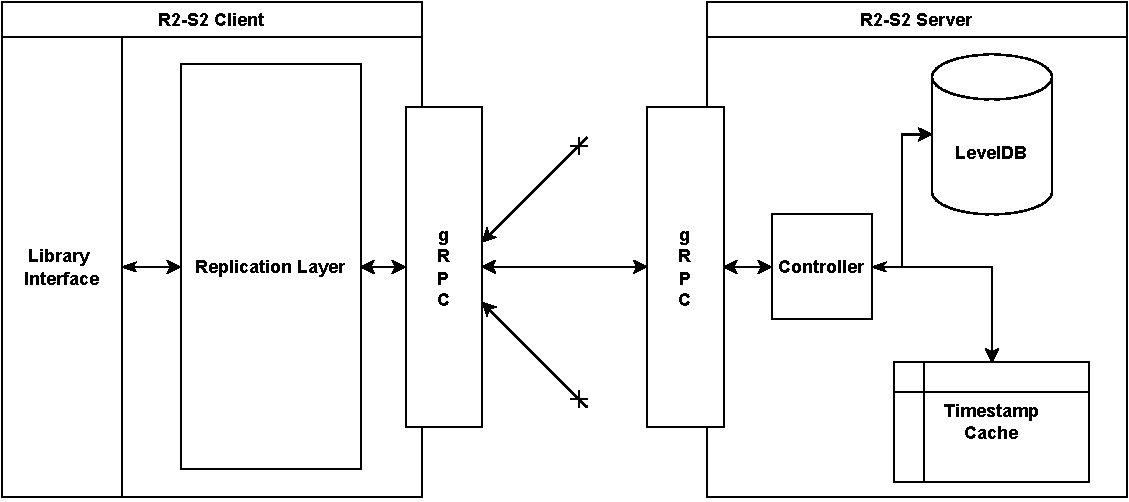
\includegraphics[width=\linewidth]{img/r2s2_arch}
    \caption{Architecture of the \ac{R2-S2}
    prototype}\label{fig:r2s2arch}
\end{figure}

The \ac{R2-S2} system is comprised of a client and several
servers, where the client is implemented as a library that
implements the replication layer and handles the connection to
and coordination of the multiple \ac{R2-S2} servers.

Each \ac{R2-S2} server consists of an RPC controller, which
handles the interface with the client. This controller manages
the server's local \ac{KVS} (in our case,
LevelDB~\cite{leveldb}). In our prototype, we chose to implement
the ABD~\cite{abd} protocol, since its read/write interface
maches perfectly with the \ac{KVS} interface we are aiming to
implmenet. One relevant aspect of ABD, and most other replication
protocols, is the notion of object versions, which are not directly supported by the
\acp{KVS}. To order concurrent writes to the same object with
different timestamps, an in memory timestamp cache is required. This
cache is populated as needed, with synchronization on the values
to order the writes to ensure that a newer value is not
overwritten by a previous one.

The overall architecture of the \ac{R2-S2} prototype is
summarized in Figure~\ref{fig:r2s2arch}.

}

%%%%%%%%%%%%%%%%%%%%%%%%%%%%%%%%%%%%%%%%%%%%%%
\subsection{Scheduling}\label{ssec:schedule}
%%%%%%%%%%%%%%%%%%%%%%%%%%%%%%%%%%%%%%%%%%%%%%

As we have covered, a good schedule is crucial to realize the
performance potential of the architecture. A \emph{schedule} is a
sequence $S$, where $S_i^j$ is the mode of operation (batch and
reply, batch and wait or sync to log) to be applied by replica
$i$ for the $j^\text{th}$ write operation. The
schedule is said to be \emph{valid} if the volatile set (i.e,
the number of batch and reply modes of operation) does not exceed
$M_R$, for every $S^j$. Thus, any valid schedule guarantees
strong persistence.

There are several approaches to scheduling. Which is preferable
is non-obvious beforehand: the schedule will be sensitive to the
particularities of the replication protocol, the deployment and
the operation load. In the preliminary evaluation in
\S~\ref{sec:r2s2evaluation} we present an
evaluation of some of the scheduling policies described
here.

At a high level, there are two types of schedules: \emph{static}
schedules, which can pre-determined ahead of time, and as such
are independent of the load the system is being subjected to; and
\emph{dynamic} schedules, which are computed on the fly and as
such can be \emph{reactive} to the load and current status of the
system. In this dissertation we will focus on static schedules,
as they are simpler and sufficient to showcase the gains from the
\ac{RR} model.

\paragraph{Constant Schedule.} A constant schedule is one where
all write operations use the same modes of operation for each
replica. In other words, all $S^j$s are equal. This schedule is,
at face value, a poor choice, since it prevents the replicas in the
critical set from ever batching. However, if the replica set is
very heterogeneous, this might be used to provide a tailored
approach to the hardware characteristics.

\paragraph{Random Schedule.} A schedule where replicas are
randomly allocated to the sync and volatile sets (based on the
sizes they need to have for the schedule to be valid).

\paragraph{Round Robin Schedule.} A schedule where the sync set
is shifted at each round. For instance, in a system with $N = 5,
M_R = 2$, replicas $0, 1, 2$ are the sync set at step $j$, and
at step $j + 1$ replicas $3, 4, 0$ become the sync set, and so
on.

\bsd{TODO: figures with schedule time diagrams}

Assuming a good random number generator, both the random and the
round robin schedules should evenly distribute the load among the
replicas. However, the random scheduler may offer less
predictable performance.

%%%%%%%%%%%%%%%%%%%%%%%%%%%%%%%%%%%%%%%%%%%%%%
\subsection{Storage Layer}\label{ssec:storage}
%%%%%%%%%%%%%%%%%%%%%%%%%%%%%%%%%%%%%%%%%%%%%%

The storage layer plays a crucial role in realizing the
performance potential of the system. It needs to efficiently support
three different types of write operations, one for each of the
different baseline approaches. It will also need to support read operations
efficiently. Figure~\ref{fig:storage_layer} shows a diagram of
the storage layer and its data-structures.

An \ac{LSM-tree} is employed as the core data structure of the storage
layer, enabling the sequential writes required for batching as
well as providing reasonable read performance. There exists a
log, used to write values that need to be synced immediately, and
an in-memory batch for values that should be batched. To further speed
up reads there is an optional in-memory object cache.

\begin{figure}[t]
    \centering
    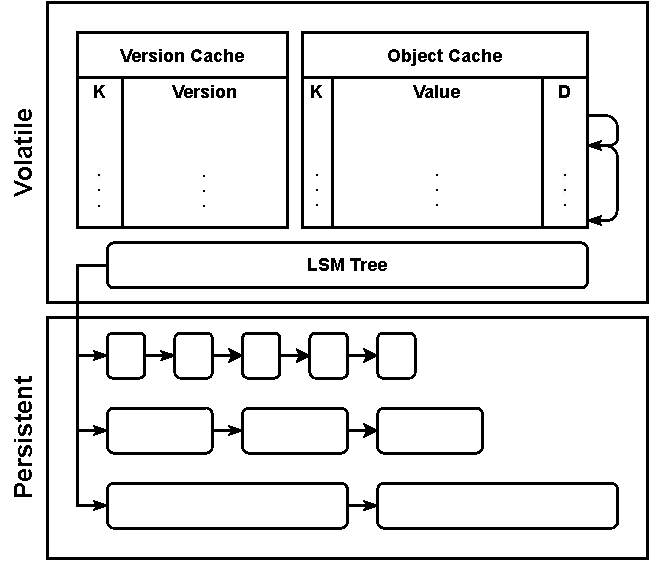
\includegraphics[width=.75\linewidth]{img/storage_layer}
    \caption{Diagram of the Storage Layer}\label{fig:storage_layer}
\end{figure}


There is an additional in-memory cache, which only stores the
object versions. This is useful because versions are a staple of
most replication protocols and several of them require reading
the current version before writing a new one. Since versions are
constant-sized and small, the capacity of the version cache can
be significantly larger than that of the object cache. This cache
is required to synchronize concurrent writes of different
versions to the same key. When the node is writing a value, it required to
check the version cache, populating it if required, where an
atomic update is executed on the version to ensure that an old
version does not override a newer version it is racing with.

With these data structures in place, the various operations
requried to implement the \ac{KVS} interface and asymmetric
syncing become quite simple. Satisfying version reads is simple:
the timestamp cache is consulted (falling back on the
\ac{LSM-tree} and log if needed). The workflow of an object read
is similar: if the object cache exists it is consulted, falling
back on the \ac{LSM-tree} and the log in the event of a miss.
Handling batch and reply writes requires placing the value
in the batch and eventually a background thread will flush the
batch into the \ac{LSM-tree}. Handling sync and reply writes
amounts to placing it in the persistent log, with this log being
compacted into the \ac{LSM-tree} at a later time by a background
thread.


%%%%%%%%%%%%%%%%%%%%%%%%%%%%%%%%%%%%%%%%%%%%%%
\section{Parametrizing the System}\label{sec:r2s2parametrization}
%%%%%%%%%%%%%%%%%%%%%%%%%%%%%%%%%%%%%%%%%%%%%%

To parametrize our system, we effectively need to choose
appropriate values for $M_R$ and $F$. We employ a data-driven
approach to this problem. Relying on real-world information about
the availability and reliability of components, we can predict
the reliability and availability of the system as a function of
$M_R$ and $F$. Choosing the adequate values becomes an exercise of
setting the desired reliability/availability and solving for $M_R$
and $F$.

The availability of the system (probability that it is available
at a particular point in time) is impacted by the availability of
the individual replicas. Let $p_c$ be the symmetric of the
availability of a replica, ie: the probability that a replica is
\emph{crashed} at a particular point in time.

The reliability (probability that the system loses data over a
given period of time) of the
system is dependent on the reliability of the underlying storage
devices and the availability of the replicas in the eager set.
Let $p_f$ be the probability that a storage device fails
(irrecoverably) in that period of time.

\new{
In order to derive the parametrization of the system, let us
begin with a simplifying assumption that all failures (both
crashes and storage device failures) are independent among all
replicas, an assumption valid for a geo-replicated deployment,
for instance. Let us first consider reliability. The probability
that all replicas in the eager set crash (and thus all the
replicas that only had the data in volatile storage lose that
data) is $p_c^{M_R}$, since $M_R$ is the size of the eager set.
To truly lose the data, the remainder of the replicas in the
write quorum would have had to suffer an irrecoverable fault in
their storage devices, which happens with probability $p^{W_Q -
M_R}$. Due to the independence of failures, we can derive the
probability that data is lost to be $p_c^{M_R} \cdot p_f^{W_Q -
M_R}$, making the reliability of the system be $1 - p_c^{M_R}
\cdot p_f^{W_Q - M_R}$. Considering availability, we know that
the system is available if a read quorum and a write quorum are
available. Due to the independence of failures, the quorums
become unavailable with probability $p_c^{R_Q}$ and $p_c^{W_Q}$,
repectively. As such, the probability that they are both
available at a given point in time is simply $1 - p_c^{\min(R_Q,
W_Q)}$.

Now let us imagine that the probability of replicas crashing
\emph{is} correlated, as is the case in a datacenter deployment.
Then, the probability of $n$ replicas crashing is the same as the
probability of a single replica crashing: $p_c$. Considering
reliability, this means that the probability of the eager set
losing its volatile state due to a crash \emph{and} the remainder
of the write quorum suffering an irrecoverable failure is $p_c
\cdot p_f^{W_Q - M_R}$. Availability is quite simpler to derive,
as if the probability of quorums of any type being unavailable is
simply $p_c$, making the availability of the system $1 - p_c$.
}


Table~\ref{tab:parametrization} summarizes the availability and
reliability of the system in these two scenarios.

\begin{table}[ht]
    \centering
    \caption{Availability and reliability in a geo-replicated
    deployment versus a datacenter deployment. $R_Q$ and $W_Q$
    are the sizes of the quorums for a parametrization with $M_R$
    tolerated rollbacks and $F$ crash faults}\label{tab:parametrization}
    \begin{tabular}{|r||c|c|}
        \hline
        & \textbf{Geo-replicated} & \textbf{Datacenter} \\ \hline
        \textbf{Availability} & $1 - p_c^{\min(R_Q, W_Q)}$ & $1 - p_c$ \\ \hline
        \textbf{Reliability}  & $1 - p_c^{M_R} \cdot p_f^{W_Q - M_R}$ & $1 - p_c \cdot p_f^{W_Q - M_R}$ \\ \hline
    \end{tabular}\label{tab:parametrization}
\end{table}


%%%%%%%%%%%%%%%%%%%%%%%%%%%%%%%%%%%%%%%%%%%%%%
\section{Implementation}\label{sec:r2s2implementation}
%%%%%%%%%%%%%%%%%%%%%%%%%%%%%%%%%%%%%%%%%%%%%%

We implemented \ac{R2-S2} using LevelDB~\cite{leveldb} as the
underlying storage layer and our own replication layer on top of
it. This was extremely helpful since LevelDB already implements
the \ac{LSM-tree}, the persistent log and the optional object cache
out of the box, and provides for two out of the three modes of
operation: batch and reply and sync and reply.

The replication layer was implemented in Rust with the request transport
being handled by gRPC~\cite{grpc}. The \ac{R2-S2} client library
provides a shim that interacts with the replication layer that
coordinates the \ac{ABD} operations. The \ac{R2-S2} server
receives requests via gRPC and manages the timestamp cache and
its embedded LevelDB instance.

The client library was implemented in approximately 2KLoC of
Rust. The server was implemented in 400LoC. The gRPC protocol
definition is comprised of 135 LoC. All the remainder driver code
for benchmarks consists of 2KLoC of Rust.

%%%%%%%%%%%%%%%%%%%%%%%%%%%%%%%%%%%%%%%%%%%%%%
\section{Evaluation}\label{sec:r2s2evaluation}
%%%%%%%%%%%%%%%%%%%%%%%%%%%%%%%%%%%%%%%%%%%%%%

\bsd{TODO}
